\chapter{Implementation and Performance Evaluation}
\label{ch:est}

Chapter~\ref{ch:method} left two fitted functions and an offline score. This chapter puts them in a cyclic program and runs the program on the seasonal mix and on one feed transient. The program is the implementation. The tables are the evaluation. Both stay inside the reduced-order plant. No number below was measured on a machine in a field.

\section{An Automated Control System}
\label{sec:sys}

\subsection{What the program is}

The control system is one cyclic executive. It does not contain a second optimizer, a vision pipeline, or a copy of the teacher. At each control step it standardizes a feature window with the training moments of \eqref{eq:std}, evaluates the status network and the command network, and writes a rate-limited command. Figure~\ref{fig:exec} is the data path. The four blocks are ordinary functions. Their only state is the window, the last command, and a fault bit.

\begin{figure}[ht]
\centering
\begin{tikzpicture}[>=Stealth,node distance=7mm,font=\small]
  \node[draw,align=center,minimum width=2.7cm,minimum height=1.15cm] (w) {window\\8 samples};
  \node[draw,align=center,right=9mm of w,minimum width=2.5cm,minimum height=1.15cm] (f) {features\\and \eqref{eq:std}};
  \node[draw,align=center,right=9mm of f,minimum width=2.6cm,minimum height=1.15cm] (n) {status net\\command net};
  \node[draw,align=center,right=9mm of n,minimum width=2.6cm,minimum height=1.15cm] (a) {rate limit\\and write};
  \draw[->] (w) -- (f);
  \draw[->] (f) -- (n);
  \draw[->] (n) -- (a);
  \node[draw,align=center,below=8mm of n,minimum width=3.4cm,minimum height=0.9cm] (g) {if confidence \(<0.55\),\\write the moisture card};
  \draw[->] (n) -- (g);
  \draw[->] (g.east) -| (a.south);
\end{tikzpicture}
\caption{The onboard path. The teacher that produced \(\mathbf{u}^\star\) is not in this figure. The confidence gate selects between the command network and the moisture card of \eqref{eq:card}.}
\label{fig:exec}
\end{figure}

The tasks and the periods are fixed in advance. Nothing in the executive is a general-purpose scheduler, because a late feature build must not be free to delay the write by an unbounded amount \cite{astrom2008}.

\begin{table}[ht]
\centering
\caption{Cyclic tasks. Periods are the rates the numerical program steps at. Budgets are operation counts, not measured times on an embedded board.}
\label{tab:tasks}
\small
\begin{tabular}{@{}lllp{4.3cm}@{}}
\toprule
Task & Period & Work & Writes \\
\midrule
Acquire & \(50\,\mathrm{ms}\) & one sample into an 8-deep window & window, fault bits \\
Features & \(200\,\mathrm{ms}\) & means, deviations, contrast, \eqref{eq:std} & \(\tilde{\mathbf{x}}\) \\
Status & \(200\,\mathrm{ms}\) & \(2885\)-parameter softmax net & label, confidence \\
Command & \(200\,\mathrm{ms}\) & \(7908\)-parameter net, \(7744\) multiply-adds & \(\hat{\mathbf{u}}\), or the card \\
Write & \(200\,\mathrm{ms}\) & clip the step to \(0.08\) on each component & the plant command \\
\bottomrule
\end{tabular}
\end{table}

A desktop timing of the command net, batched in the same NumPy implementation that trained it, is well under a millisecond per window. That figure is not a board measurement and is not used as one. The operation count is the fact the period has to dominate. Seven thousand multiply-adds are two orders of magnitude inside a \(200\,\mathrm{ms}\) step on any processor that would be chosen to host this net. The reason for the cap is the rate limit and the window, not the arithmetic. The teacher, by contrast, is a grid plus an iterative solve and is not a candidate for the step. That difference is why Problem~2 is an imitation problem.

\subsection{Channels the executive consumes}

Table~\ref{tab:chan} is the measurement vector of requirement R1, written as channels rather than as a wiring diagram. The four axial stations are the installed set \(\{1,4,5,8\}\). The other channels are the scalars of Section~\ref{sec:place}. Sampling faster than the feature task is only so the window has eight distinct values; the executive never acts at the sample rate.

\begin{table}[ht]
\centering
\caption{Channels read by the executive. ``Used'' is the rate at which a new value enters the decision.}
\label{tab:chan}
\begin{tabular}{@{}llc@{}}
\toprule
Channel & Role & Used at \\
\midrule
Loads at stations \(1,4,5,8\) & shape, level, peak & \(20\,\mathrm{Hz}\) window \\
Shaft torque & level, redundant with the loads & \(20\,\mathrm{Hz}\) \\
Housing vibration & intensity check & \(20\,\mathrm{Hz}\) \\
Sieve-loss proxy & cleaner term & \(20\,\mathrm{Hz}\) \\
Return flow & accompanies sieve loss & \(20\,\mathrm{Hz}\) \\
Shaft power & accompanies specific energy & \(20\,\mathrm{Hz}\) \\
Moisture & disturbance and card input & \(1\,\mathrm{Hz}\) \\
Offered feed & disturbance & \(20\,\mathrm{Hz}\) \\
\bottomrule
\end{tabular}
\end{table}

The command write is four normalized setpoints. Intensity, residence, cleaning, and feed admission remain the interface of Chapter~\ref{ch:back}. The executive does not convert them to a rotor speed or a sieve angle. That conversion is a property of a particular machine and is outside the claim. The rate limit of \(0.08\) per component per \(200\,\mathrm{ms}\) is the claim: a step that the numerical transient is required to obey, so a jump in the network output cannot appear as a jump in the plant.

\subsection{Faults, and the direction of the fallback}

A missing axial station is dropped from the contrast and from the coefficient of variation, and the command is held for that step. If two or more of the four installed stations are missing, the write is the moisture card until the channels return. A missing moisture reading holds the last moisture and raises a fault bit. It does not invent a dry crop, because the card would then move the wrong way. A status confidence below \(0.55\) selects the card for that step. On the test windows this gate fires on \(2.5\%\) of rows. The seasonal runs and the slug in Section~\ref{sec:eval} do not inject missing channels, and they do not take the gate's credit. They are the networks with a full window. The gate is specified so that a low-confidence window has a defined output; it is not secretly responsible for the loss reduction in the tables.

The card is the fallback in every one of these cases, rather than the fixed setting or a zero command. The card is a function of moisture, it is always defined, and Chapter~\ref{ch:method} already measured it. Falling back to a command that has not been measured would make the fault logic a third controller.

\subsection{The season the program is scored on}

Eight steady points and one transient are the evaluation. The points, the feeds, the moistures, and the weights are in Table~\ref{tab:points}. The weights sum to one. They describe a wheat-heavy mix with a real rice and soybean share. They are not a yield census. The transient is wheat at moisture \(0.17\), with offered feed
\begin{equation}
q(t) = 5.0 + 3.2\exp\!\big(-{\textstyle\frac12}((t-12)/2.2)^2\big)
\label{eq:slug}
\end{equation}
from \(t=0\) to \(t=26\,\mathrm{s}\), sampled every \(0.2\,\mathrm{s}\). The crest is about \(8.2\,\mathrm{kg\,s^{-1}}\). The network starts on the card, fills the window, and is then rate-limited. The fixed command and the card are run on the same \(q(t)\) with no rate limit, because they do not move.

\begin{table}[ht]
\centering
\caption{Seasonal points. Feed is offered biomass. Weights sum to one.}
\label{tab:points}
\begin{tabular}{@{}lcccc@{}}
\toprule
Point & Crop & Feed (\(\mathrm{kg\,s^{-1}}\)) & Moisture & Weight \\
\midrule
Wheat, nominal & wheat & 6.0 & 0.145 & 0.22 \\
Wheat, wet & wheat & 6.0 & 0.220 & 0.14 \\
Wheat, dry and heavy & wheat & 8.0 & 0.120 & 0.12 \\
Wheat, light & wheat & 3.5 & 0.160 & 0.10 \\
Rice, nominal & rice & 5.0 & 0.180 & 0.14 \\
Rice, wet & rice & 6.4 & 0.250 & 0.12 \\
Soybean, nominal & soybean & 4.5 & 0.130 & 0.10 \\
Soybean, wet & soybean & 4.2 & 0.180 & 0.06 \\
\bottomrule
\end{tabular}
\end{table}

\section{Performance Evaluation}
\label{sec:eval}

\subsection{Seasonal means}

Table~\ref{tab:season} is the weighted mean of the eight points. Five policies are columns because five different questions would otherwise be collapsed. Fixed is the setting an operator leaves alone. The card is the moisture schedule \eqref{eq:card}. Linear is the least-squares imitator. Network is the deep imitator in the executive, without the rate limit, because these points are steady. Oracle is the teacher with the true disturbance. The network column is the one Problem~2 asked for. The oracle column is the ceiling of the imitation, not a field target.

\begin{table}[ht]
\centering
\caption{Weighted seasonal means. Loss terms and impurity and breakage are percent. Energy is \(\mathrm{kWh\,t^{-1}}\). Power is kilowatts.}
\label{tab:season}
\begin{tabular}{@{}lrrrrr@{}}
\toprule
Quantity & Fixed & Card & Linear & Network & Oracle \\
\midrule
Grain loss (\%) & 2.85 & 2.50 & 1.88 & 1.80 & 1.78 \\
Unthreshed (\%) & 0.93 & 0.76 & 0.53 & 0.49 & 0.47 \\
Free grain (\%) & 1.06 & 0.93 & 0.77 & 0.75 & 0.74 \\
Sieve loss (\%) & 0.86 & 0.82 & 0.58 & 0.57 & 0.57 \\
Recovery (\%) & 97.15 & 97.50 & 98.07 & 98.13 & 98.22 \\
Impurity (\%) & 1.17 & 1.20 & 1.50 & 1.50 & 1.50 \\
Breakage (\%) & 1.04 & 1.17 & 1.43 & 1.49 & 1.51 \\
Specific energy & 1.41 & 1.47 & 1.60 & 1.63 & 1.64 \\
Load CV & 0.140 & 0.127 & 0.109 & 0.104 & 0.105 \\
Peak load (N) & 969 & 952 & 930 & 928 & 929 \\
Stability \(S\) & 0.686 & 0.696 & 0.702 & 0.701 & 0.700 \\
Shaft power (kW) & 13.1 & 13.6 & 14.9 & 15.2 & 15.2 \\
\bottomrule
\end{tabular}
\end{table}

Grain loss falls from \(2.85\%\) at the fixed setting to \(2.50\%\) on the card and to \(1.80\%\) with the network. The teacher sits at \(1.78\%\). The network is within \(0.03\) points of the teacher and \(0.08\) points under the linear imitator. Recovery moves with loss because the feed trim stays open: the seasonal recovery and the complement of seasonal loss differ by less than a tenth of a point in every learned column. The network is not buying the table by refusing crop.

The prices move in the direction \(J\) told them to move. Specific energy rises from \(1.41\) to \(1.63\,\mathrm{kWh\,t^{-1}}\), shaft power from \(13.1\) to \(15.2\,\mathrm{kW}\), impurity from \(1.17\%\) to \(1.50\%\), and breakage from \(1.04\%\) to \(1.49\%\). The teacher's own column is \(1.64\), \(1.50\%\), and \(1.51\%\). The network is copying the teacher's purchase, not inventing a cheaper one. Stability rises from \(0.686\) to \(0.701\), which is the floor. A mean of \(0.701\) can hide a point that is far under the floor and another that is far over it. The point table is where that question is answered.

The card deserves a plain reading. It beats the fixed setting on the mean, by \(0.35\) points of loss, and it spends a little energy and a little breakage to do it. It is a real policy. The network's further \(0.70\) points are the part of the problem the card cannot see: feed, packing, and the load shape.

\subsection{Point by point}

Table~\ref{tab:pointsfull} gives loss, stability, and specific energy at each point for the fixed setting, the card, the network, and the teacher. The linear map is omitted here because its seasonal mean is already in Table~\ref{tab:season} and the point-level story is about whether the network tracked the teacher where the card fails.

\begin{table}[ht]
\centering
\caption{Loss (\%), stability \(S\), and specific energy at each seasonal point.}
\label{tab:pointsfull}
\small
\setlength{\tabcolsep}{4pt}
\begin{tabular}{@{}lrrrrrrrrrrrr@{}}
\toprule
& \multicolumn{3}{c}{Fixed} & \multicolumn{3}{c}{Card} & \multicolumn{3}{c}{Network} & \multicolumn{3}{c}{Oracle} \\
\cmidrule(lr){2-4}\cmidrule(lr){5-7}\cmidrule(lr){8-10}\cmidrule(lr){11-13}
Point & \(L\) & \(S\) & \(e\) & \(L\) & \(S\) & \(e\) & \(L\) & \(S\) & \(e\) & \(L\) & \(S\) & \(e\) \\
\midrule
Wheat nom. & 2.46 & 0.71 & 1.33 & 2.44 & 0.72 & 1.33 & 1.57 & 0.70 & 1.55 & 1.54 & 0.70 & 1.56 \\
Wheat wet & 3.40 & 0.65 & 1.54 & 2.61 & 0.67 & 1.70 & 2.07 & 0.70 & 1.80 & 2.01 & 0.70 & 1.82 \\
Wheat heavy & 2.65 & 0.64 & 1.29 & 2.85 & 0.64 & 1.25 & 1.57 & 0.72 & 1.54 & 1.96 & 0.70 & 1.39 \\
Wheat light & 1.93 & 0.76 & 1.32 & 1.83 & 0.77 & 1.35 & 1.50 & 0.70 & 1.46 & 1.52 & 0.70 & 1.45 \\
Rice nom. & 3.00 & 0.72 & 1.46 & 2.65 & 0.73 & 1.54 & 1.99 & 0.69 & 1.69 & 1.86 & 0.70 & 1.73 \\
Rice wet & 4.99 & 0.54 & 1.70 & 3.37 & 0.56 & 1.94 & 2.65 & 0.70 & 2.07 & 2.27 & 0.70 & 2.19 \\
Soy nom. & 1.83 & 0.76 & 1.23 & 1.90 & 0.76 & 1.21 & 1.41 & 0.70 & 1.34 & 1.42 & 0.70 & 1.33 \\
Soy wet & 2.06 & 0.76 & 1.36 & 1.84 & 0.76 & 1.43 & 1.56 & 0.71 & 1.49 & 1.54 & 0.70 & 1.51 \\
\bottomrule
\end{tabular}
\end{table}

Three rows carry the argument. The others are the same pattern at a smaller scale.

On nominal wheat the card and the fixed setting are the same policy for practical purposes, loss \(2.46\%\) and \(2.44\%\), because the card was written to pass near the fixed setting at moderate moisture. The network lowers loss to \(1.57\%\), against the teacher's \(1.54\%\), and raises energy from \(1.33\) to \(1.55\,\mathrm{kWh\,t^{-1}}\). Stability was already at the floor and stays there. The command the network writes is \((0.69,\ 0.55,\ 0.65,\ 1.00)\), against the teacher's \((0.70,\ 0.55,\ 0.65,\ 1)\). Intensity and cleaning rise. Residence rises a little. The feed trim does not move.

On dry, heavy wheat the card is worse than the fixed setting: loss \(2.85\%\) against \(2.65\%\), energy slightly down. Low moisture tells the card to ease off, and the heavy feed is invisible to it. The teacher goes the other way on residence, to \(0.59\), and holds intensity at \(0.50\), with loss \(1.96\%\) and energy \(1.39\). The network overshoots that instruction. It writes \((0.59,\ 0.71,\ 0.68,\ 1)\), loss \(1.57\%\), energy \(1.54\), breakage \(1.63\%\) against the teacher's breakage of \(1.27\%\). Loss looks better than the teacher and the objective does not, because breakage and energy were the terms the teacher refused to spend. This is the row where imitation error is visible as a purchase, not as a random residual. It is also the row that shows why a loss-only table would have ranked the network above the teacher and been wrong about \(J\).

On wet rice the fixed setting loses \(4.99\%\), sits at stability \(0.54\), and peaks at \(1441\,\mathrm{N}\), which is over the blockage line of \(1411\,\mathrm{N}\). The card cuts loss to \(3.37\%\) and leaves stability at \(0.56\). The teacher raises residence to \(0.85\) and intensity to \(0.63\), cuts loss to \(2.27\%\), brings the peak down to \(1163\,\mathrm{N}\), and pays with breakage \(3.36\%\) and energy \(2.19\,\mathrm{kWh\,t^{-1}}\). The network writes \((0.56,\ 0.80,\ 0.66,\ 1)\). Loss is \(2.65\%\), stability \(0.70\), peak load \(1182\,\mathrm{N}\), breakage \(2.96\%\), energy \(2.07\). It reaches the floor and it does not reach the teacher's loss. The gap of \(0.38\) points is the largest point-level gap in the table. The load coefficient of variation on this row falls from \(0.157\) at the fixed setting to \(0.047\) under the network. That is the shape term doing the work the card cannot do, and it is why the middle-and-end placement is in the feature vector even though two stations already classify the label.

On light wheat the fixed setting is already above the floor, at \(0.76\). The teacher spends the margin down to \(0.70\), lowers residence to \(0.37\), and cuts loss from \(1.93\%\) to \(1.52\%\). The network does the same thing: residence \(0.38\), loss \(1.50\%\), stability \(0.70\). Extra residence is not a universal command. The objective's hinge is the reason. Above \(0.70\), further calmness is unpaid, and a light crop should not be held longer for a calmness the cost does not buy.

Feed admission stays at \(1\), or within \(0.01\) of \(1\), on every seasonal point and for both the network and the teacher. The trim is in the command vector because the plant allows it and because a policy that used it would be visible in the recovery column. Neither the teacher nor the imitator needs it on this mix. The blockage hinge is met by residence and intensity instead. A heavier point than wet rice could move the trim. No such point is in the weighted mean, and none is added after the fact.

\subsection{The feed transient}

The slug of \eqref{eq:slug} asks whether a rate-limited network, which at \(t=0\) is still equal to the card, gives the steady-state gain back when the feed rises for a few seconds. Figure~\ref{fig:slug} is the peak station load. Table~\ref{tab:slug} is the same run at the crest and at the two shoulders.

\begin{figure}[ht]
\centering
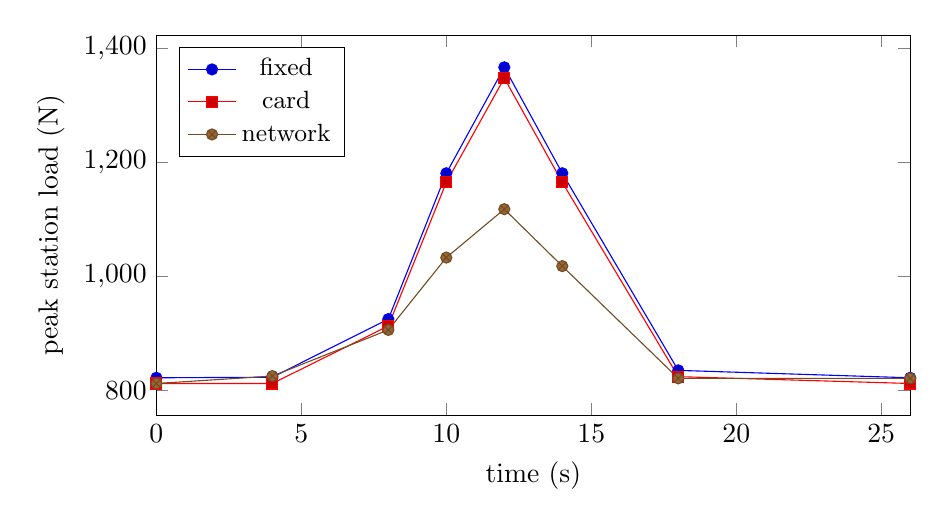
\begin{tikzpicture}
\begin{axis}[
  width=0.92\textwidth,
  height=6.4cm,
  xlabel={time (s)},
  ylabel={peak station load (N)},
  xmin=0, xmax=26,
  legend style={font=\small,at={(0.03,0.97)},anchor=north west},
]
\addplot coordinates {
(0,822) (4,823) (8,925) (10,1181) (12,1367) (14,1181) (18,835) (26,822)
};
\addplot coordinates {
(0,812) (4,812) (8,913) (10,1165) (12,1348) (14,1165) (18,824) (26,812)
};
\addplot coordinates {
(0,812) (4,825) (8,906) (10,1033) (12,1118) (14,1018) (18,821) (26,821)
};
\legend{fixed,card,network}
\end{axis}
\end{tikzpicture}
\caption{Peak station load through the wheat feed transient at moisture \(0.17\). The offer peaks near \(8.2\,\mathrm{kg\,s^{-1}}\) at \(t=12\,\mathrm{s}\). The network is rate-limited and starts on the card.}
\label{fig:slug}
\end{figure}

\begin{table}[ht]
\centering
\caption{Wheat transient at moisture \(0.17\). Loss is percent. Peak load is newtons.}
\label{tab:slug}
\begin{tabular}{@{}rrrrrrrr@{}}
\toprule
& & \multicolumn{2}{c}{Fixed} & \multicolumn{2}{c}{Card} & \multicolumn{2}{c}{Network} \\
\cmidrule(lr){3-4}\cmidrule(lr){5-6}\cmidrule(lr){7-8}
\(t\) (s) & Feed & Loss & Peak & Loss & Peak & Loss & Peak \\
\midrule
0 & 5.00 & 2.43 & 822 & 2.22 & 812 & 2.22 & 812 \\
4 & 5.00 & 2.43 & 823 & 2.23 & 812 & 1.44 & 825 \\
8 & 5.61 & 2.59 & 925 & 2.37 & 913 & 1.55 & 906 \\
12 & 8.20 & 3.19 & 1367 & 2.92 & 1348 & 1.81 & 1118 \\
18 & 5.08 & 2.45 & 835 & 2.24 & 824 & 1.33 & 821 \\
26 & 5.00 & 2.43 & 822 & 2.22 & 812 & 1.49 & 821 \\
\bottomrule
\end{tabular}
\end{table}

At \(t=0\) the network has not moved, and its loss equals the card. By \(t=4\,\mathrm{s}\), still before the crest, loss is \(1.44\%\) and the command has walked to about \((0.74,\ 0.58,\ 0.63,\ 1)\). At the crest the fixed peak is \(1367\,\mathrm{N}\) and the network peak is \(1118\,\mathrm{N}\). Fixed loss is \(3.19\%\) and network loss is \(1.81\%\). The load coefficient of variation at the crest is \(0.141\) for the fixed command and \(0.026\) for the network: residence has risen to \(0.84\), which is the same direction the teacher used on wet, heavy steady points. Minimum stability over the twenty-six seconds is \(0.586\) for the fixed command, \(0.597\) for the card, and \(0.701\) for the network. Mean loss over the transient is \(2.59\%\), \(2.38\%\), and \(1.48\%\).

The rate limit is what makes the four-second delay in Table~\ref{tab:slug} a real delay rather than a skipped sample. A command that jumped from the card to the crest command in one step would have produced the same crest numbers and would have violated the write rule in Table~\ref{tab:tasks}. The plotted run does not do that. From \(t=4\) to \(t=12\) residence moves from \(0.58\) to \(0.84\) while the feed is rising, which is several capped steps, not one.

\subsection{What the evaluation does and does not establish}

The evaluation establishes four comparisons on this plant, at the published weights of \eqref{eq:J}, with seed \(7\).

The status network on the installed placement is more accurate than a linear softmax on the features the placement makes, and the margin is in the spatial and the rare classes. That result belongs to Chapter~\ref{ch:method} and is not re-litigated by the loss tables. A season can look good while the labeler is weak, because the command net never reads the label.

The command network reproduces the teacher's seasonal loss to \(0.03\) points and the teacher's energy, impurity, and breakage to a few hundredths. A linear imitator of the same teacher recovers most of the same gain and leaves \(0.08\) points more loss on the seasonal mean. Depth is a small advantage on the command once the features exist. It is not zero on this mix, and it is not the reason the card loses.

The moisture card is a lawful baseline. It helps on wet wheat and on wet rice, and it hurts on dry, heavy wheat. Any summary that reports only the seasonal mean of the card will call it a modest improvement and will miss the row it gets backwards.

The stability floor is met as a seasonal mean and as a minimum along the tested transient. It is not met as a hard constraint on every random test window: Chapter~\ref{ch:method} recorded that \(30\%\) of those windows still fall just under \(0.70\) after imitation, against \(0.4\%\) for the teacher. The tenth percentile on that mixture is \(0.693\). The executive does not project \(\hat{\mathbf{u}}\) back onto \(\{S\ge 0.70\}\). Doing so would require the plant inside the step, which is the teacher again. The gap is the price of a pure function evaluation, and it should be read as a gap.

The evaluation does not establish a field loss of \(1.80\%\). The plant was built so that a fixed command would sit in a published band of axial loss and specific energy, and so that feed and moisture would interact. A different breakage weight would move the dry-heavy overshoot and the wet-rice purchase. The same comparison, at these weights, is what the tables are for: a fixed setting and a moisture card, against a network that imitates a cost in which those purchases are explicit, with the teacher present in the last column so the imitation can be seen to succeed and, on two rows, to miss.
